\documentclass[12pt,a4paper]{report}

\usepackage{titlesec}
\usepackage{hyperref}

% Custom centered chapter format for front matter
\newcommand{\chaptercenter}[1]{%
  \titleformat{\chapter}[display]
    {\normalfont\bfseries\centering\fontsize{24}{28}\selectfont}
    {}
    {0pt}
    {} % No label
  \chapter*{#1} % Print chapter title
  \titleformat{\chapter}[display] % Restore main format
    {\normalfont\huge\bfseries}
    {\chaptertitlename\ \thechapter}
    {-1pt}
    {\huge}
  \titlespacing*{\chapter}{0pt}{15pt}{20pt} % Restore spacing
}

\usepackage{enumitem}
\usepackage{enumitem} % put in preamble
\usepackage{tabularx}  % for auto-adjustable tables
\renewcommand{\arraystretch}{1.3} % row height
\usepackage{adjustbox}
\usepackage{setspace}
\usepackage{geometry}
\usepackage{graphicx}
\usepackage{tocloft}
\usepackage{newtxtext} % Times New Roman
\usepackage{fancyhdr}
\usepackage{array}
\usepackage{longtable}
\usepackage{float}
\usepackage[utf8]{inputenc}
\usepackage{booktabs}
\usepackage{amsmath}
\usepackage{enumitem}
\usepackage{hyperref}
\usepackage[numbers]{natbib}
\usepackage{placeins}
\usepackage{newtxmath}
\usepackage{adjustbox}
\usepackage{subcaption}
\usepackage[font=footnotesize,labelfont=bf,justification=centering]{caption}
\setcounter{secnumdepth}{3}
\setcounter{tocdepth}{3}

\geometry{margin=1in}
\setstretch{1.5}

% Page style setup
\pagestyle{plain} % Default to plain style (no header line) for front matter
\fancyhf{}
\renewcommand{\headrulewidth}{0.4pt} % Horizontal line in header
\cfoot{\thepage} % Page number in center footer for all pages

% Define fancy style for main content
\fancyhead[R]{\leftmark} % Chapter name in header (right)
\fancyfoot[C]{\textit{Department of Computer Engineering}} % Center footer
\fancyfoot[R]{\textit{\thepage}} % Right-aligned italic page number
\renewcommand{\chaptermark}[1]{\markboth{#1}{}} % Store chapter name for header
\renewcommand{\sectionmark}[1]{} % Ignore section name for header

% Switch to fancy style only for numbered chapters
\let\oldchapter\chapter
\renewcommand{\chapter}{\ifnum\value{chapter}>0 \clearpage\pagestyle{fancy}\fi\oldchapter}

% Roman page numbering for front matter
\pagenumbering{roman}

% Define title formats for front matter (centered for unnumbered chapters)
\titleformat{\chapter}[display]
{\normalfont\bfseries\centering\fontsize{24}{28}\selectfont}
{}
{0pt}
{}

\titleformat{\section}
{\normalfont\bfseries\fontsize{24}{28}\selectfont}
{}
{0pt}
{}

% For left aligned sections like Abstract, Contents etc.
\newcommand{\sectionleft}[1]{%
    \vspace*{1cm}%
    {\raggedright\bfseries\fontsize{24}{28}\selectfont #1\par}
    \vspace{1cm}
}

% Redefine title formats for main content
\titleformat{\section}
  {\normalfont\Large\bfseries} % Bold section headings
  {\thesection}{1em}{}
\titleformat{\subsection}
  {\normalfont\large\bfseries} % Bold subsection headings
  {\thesubsection}{1em}{}

\titleformat{\chapter}[display]
  {\normalfont\huge\bfseries}
  {\chaptertitlename\ \thechapter}
  {-1pt}
  {\huge}
\titlespacing*{\chapter}{0pt}{15pt}{20pt} % Reduced space above chapter title


\usepackage{geometry}
\geometry{margin=1in}
\usepackage{longtable}
\usepackage{array}
\renewcommand{\arraystretch}{1.3} % row height

\begin{document}

%-------------------- Title Page ---------------------
\begin{titlepage}
 
    \centering
    \vspace{1cm}
    {\Huge \bfseries Privacy Preserving LLM for Financial Data \par}
    \vspace{1.5cm}
    {\Large \bfseries STAGE-I - PROJECT REPORT \par}
    \vspace{1.5cm}

    \textbf{By}
    

    \begin{center}
    {\large
    \begin{tabular}{l l}
    Anurag Gurunath Mohit & 122A1017 \\[2pt]
    Arjunan Swamynathan   & 122A1019 \\[2pt]
    Krishant Arivalagan   & 122A1049 \\[2pt]
    Omkar Rajesh Choughule & 122A1069
    \end{tabular}
    }
    \end{center}

    \vfill
    {\large Under the guidance of \\[6pt]
    Ms.Prachi Shahane}

    \vspace{1cm}
        
\includegraphics[width=0.25\textwidth]{sies_gst_logo.png}\\[1em]

    {\large Submitted in partial fulfillment for the degree of \\[6pt]
    \textbf{Bachelor of Engineering in Computer Engineering}}

    \vspace{1cm}
    {\large Department of Computer Engineering \\ SIES Graduate School of Technology \\ Nerul, Navi Mumbai -- 400706 \\ Academic Year 2025--2026}
\end{titlepage}

\newpage

%-------------------- Certificate ---------------------
\chaptercenter{Certificate}
\thispagestyle{plain}
This is to certify that this is a bonafide record of \textbf{Project Stage-I} of the project titled \textbf{``Privacy Preserving LLM using Financial Data''} carried out by the following students of final year. 
\vspace{0.5cm}

\begin{center}
\begin{tabular}{ll}
    Anurag Gurunath Mohit \hfill & 122A1017 \\
    Arjunan Swamynathan \hfill & 122A1019 \\
    Krishant Arivalagan \hfill & 122A1049 \\
    Omkar Rajesh Choughule \hfill & 122A1069 \\
\end{tabular}
\end{center}
\vspace{0.3cm}
The report is submitted in partial fulfillment of the degree course of Bachelor of Engineering in Computer Engineering, of University of Mumbai during the academic year 2025-2026.

\begin{center}
\begin{tabular}{>{\centering\arraybackslash}p{5cm} >{\centering\arraybackslash}p{5cm} >{\centering\arraybackslash}p{5cm}}
    Ms.Prachi Shahane & Dr. Aparna Bannore & Dr. K. Lakshmisudha \\
    Internal Guide & Head of Department & Principal \\
\end{tabular}
\end{center}
We have examined this report as per University requirements at SIES Graduate School of Technology, Nerul (E), Navi Mumbai on \underline{\hspace{5cm}} \\


\begin{flushright}
Name of External Examiner: \underline{\hspace{5cm}} \\
\vspace{0.5cm}
Signature: \underline{\hspace{5cm}} \\[1cm]

Name of Internal Examiner: \underline{\hspace{5cm}} \\
\vspace{0.5cm}
Signature: \underline{\hspace{5cm}}
\end{flushright}

\vspace{1cm}

\noindent
Date: \\
Place:
\newpage

%-------------------- Declaration ---------------------
\chaptercenter{Declaration}
\thispagestyle{plain}
\vspace{1cm}

I declare that this written submission represents my ideas in my own words and where others’ ideas or words have been included, I have adequately cited and referenced the original sources.
I also declare that I have adhered to all principles of academic honesty and integrity and have not misrepresented or fabricated or falsified any idea/data/fact/source in my submission.
I understand that any violation of the above will be cause for disciplinary action by the Institute and can also evoke penal action from the sources which have thus not been properly cited or from whom proper permission has not been taken when needed.
\vspace{1cm}

\begin{center}
\begin{tabular}{lll}
    Anurag Gurunath Mohit \hfill & 122A1017 \hfill & \underline{\hspace{3cm}} \\
    Arjunan Swamynathan \hfill & 122A1019 \hfill & \underline{\hspace{3cm}} \\
    Krishant Arivalagan \hfill & 122A1049 \hfill & \underline{\hspace{3cm}} \\
    Omkar Rajesh Choughule \hfill & 122A1069 \hfill & \underline{\hspace{3cm}} \\
\end{tabular}
\end{center}

\vspace{1cm}

Date:

\newpage

%-------------------- Acknowledgement ---------------------
\chaptercenter{Acknowledgement}
\thispagestyle{plain}
\vspace{1cm}

We wish to express our deep sense of gratitude and thank our Internal Guide, Ms.Prachi Shahane for her guidance, help, and useful suggestions, which helped in completing our project work in time.
We are also extremely grateful to our Project coordinator Dr. Arathi Boyanapalli for her guidance provided whenever required.
We also thank our HOD Dr. Aparna Bannore for her support in completing the project.
We also thank our Principal Dr. K. Lakshmisudha for extending support to carry out this project.
Also, we would like to thank the entire faculty of the Computer Engineering department for their valuable ideas and timely assistance in this project.
Last but not the least, we would like to thank our teaching and non-teaching staff members of our college for their support in facilitating timely completion of this project.
\vspace{0.5cm}

\begin{flushright}
    Project Team \\
    Anurag Gurunath Mohit \\
    Arjunan Swamynathan \\
    Krishant Arivalagan \\
    Omkar Rajesh Choughule
\end{flushright}

\newpage

%-------------------- Abstract ---------------------
\sectionleft{Abstract}
\thispagestyle{plain}


\textbf \\ Financial institutions and data owners are increasingly interested in using Large Language Models (LLMs) for tasks such as risk analysis, customer support automation, automated reporting, and fraud detection. However, the highly sensitive nature of financial data (account details, transaction histories, personally identifiable information) demands privacy-aware solutions. This project develops a Privacy-Preserving LLM for Finance that allows model training and inference while minimizing leakage of sensitive information. The system combines federated learning, differential privacy, secure aggregation, and encrypted inference to train and deploy a domain-adapted LLM on financial text and structured records. We demonstrate the approach on synthetic and real-world-like financial datasets, evaluate model utility vs. privacy trade-offs, and provide deployment guidelines for banks and fintechs.


\newpage

%-------------------- Table of Contents (Manual Table) ---------------------
\begin{tabular}{|c|l|c|}
\hline
\textbf{Chapter} & \textbf{Title} & \textbf{Page Nos.} \\ \hline
1 & Introduction & 1-3 \\ \hline
  & 1.1 Overview & 1 \\ \hline
  & 1.2 Need of the Project & 1 \\ \hline
  & 1.3 Objectives & 2 \\ \hline
  & 1.4 Scope and Limitations & 2 \\ \hline
  & 1.5 Significance of the Project & 3 \\ \hline
  & 1.6 Organization of the Report & 3 \\ \hline

2 & Literature Survey & 4-7 \\ \hline
  & 2.1 Survey of Existing System & 5 \\ \hline
  & 2.2 Gap Analysis & 6 \\ \hline

3 & Proposed System & 8-10\\ \hline
  & 3.1 Overview and Block Diagram Explanation & 8 \\ \hline
  & 3.2 Components of the System & 9 \\ \hline

4 & Design and Methodology & 11-14 \\ \hline
  & 4.1 Working Model  & 11\\ \hline
  & 4.2 Methodology  & 13 \\ \hline

5 & Results & 15-17 \\ \hline
  & 5.1 System Output and Diagnostics & 15 \\ \hline
  & 5.2 Comparative Impact of Federated Learning & 16 \\ \hline

6 & Planned Tasks for Next Phase & 18-19 \\ \hline
7 & Conclusion & 20\\ \hline
8 & References & 21-23 \\ \hline
9 & Plagiarism Report & 24\\ \hline
10 & Project Competition Certificates & 25\\ \hline
\end{tabular}

\newpage

%-------------------- List of Figures (Manual Table) ---------------------
\section*{List of Figures}
\thispagestyle{plain}

\vspace{0.5cm}

\begin{table}[h!]
\centering
\begin{tabular}{|c|p{0.5\textwidth}|c|}
\hline
\textbf{Figure No.} & \centering\textbf{Figure Caption} & \textbf{Page No.} \\
\hline
3.1 & Block Diagram of the Proposed Federated Learning System & 8 \\
\hline
4.1 & System Flowchart Based on Block Diagram and Algorithm & 12 \\
\hline
5.1 & Comparative Impact of Federated Learning across Finance AI Metrics & 20 \\
\hline
5.2 & User Interface Screens — Login and Dashboard & 21 \\
\hline
9.1 & Plagiarism Report & 24 \\
\hline
10.1 & Project Competition Certificates of Team \space \space \space Members & 25 \\
\hline
\end{tabular}
\caption{List of Figures}
\end{table}

\newpage

%-------------------- List of Tables (Manual Table) ---------------------
\sectionleft{List of Tables}
\thispagestyle{plain}

\vspace{0.5cm}
\begin{center}
\begin{tabular}{|c|p{10cm}|c|}
\hline
\textbf{Table No.} & \textbf{Table Caption} & \textbf{Page No.} \\
\hline
2.1 & Literature Survey Table & 4 - 12 \\
\hline
\end{tabular}
\end{center}

\newpage

%-------------------- List of Abbreviations ---------------------
\sectionleft{List of Abbreviations}
\thispagestyle{plain}

\vspace{0.5cm}
\begin{center}
\begin{tabular}{|c|p{13cm}|}
\hline
LLM & Large Language Model \\
\hline
DP & Differential Privacy \\
\hline
FL & Federated Learning \\
\hline
HE & Homomorphic Encryption \\
\hline
MPC & Multi-Party Computation \\
\hline
SMC & Secure Multi-party Computation \\
\hline
PII & Personally Identifiable Information \\
\hline
GDPR & General Data Protection Regulation \\
\hline
API & Application Programming Interface \\
\hline
NLP & Natural Language Processing \\
\hline
\end{tabular}
\end{center}

\newpage

%-------------------- Main Content Starts Here ---------------------
% The main report body with Arabic page numbering
\clearpage
\pagenumbering{arabic}

% Chapter 1: Introduction
\chapter{Introduction}
\section{Overview}
In the financial sector, data security and confidentiality are of utmost importance. Financial institutions generate vast amounts of sensitive information such as transaction logs, credit scores, investment portfolios, and customer records. With the growing popularity of Large Language Models (LLMs) for tasks such as document summarization, fraud detection, and automated financial advisory, ensuring privacy during model training and deployment has become critical.

\textbf \\This project focuses on developing a Privacy-Preserving Large Language Model (PP-LLM) for financial data. The model aims to perform intelligent text-based tasks while adhering to strict privacy guarantees. The framework leverages Differential Privacy (DP) and Federated Learning (FL) to prevent leakage of confidential financial information during training or inference.

\section{Problem Statement}
Financial data is highly sensitive, containing personally identifiable information (PII), account numbers, and account balances, and its sharing is strictly regulated by laws such as GDPR and local banking regulations. At the same time, financial institutions seek to leverage state-of-the-art Large Language Models (LLMs) to enhance services like fraud detection, risk assessment, and automated reporting, without compromising customer privacy. Existing approaches often either reduce model accuracy or rely on a centralized trusted party, which can expose sensitive information. Therefore, it is essential to develop a practical and privacy-preserving framework that maintains regulatory compliance while effectively balancing model performance and usability, enabling the secure collaborative training and deployment of LLMs among multiple financial organizations. 



\section{Objectives}
\begin{itemize}
    \item Design a privacy-preserving training pipeline for LLMs applicable to financial text and structured records.
    \item Implement differential privacy to bound information leakage.
    \item Integrate federated learning and secure aggregation so multiple institutions can jointly improve a global model without sharing raw data.
    \item Support privacy-preserving inference (encrypted inference / client-side masking) for production use.
    \item Evaluate utility-privacy trade-offs and system performance (latency, throughput).
\end{itemize}

\section{Scope and Limitations}
\textbf{Scope:} Domain adaptation of moderately sized LLMs (e.g., open-source LLMs in the range of 100M–1B parameters) for finance-specific tasks, deployment-ready inference with privacy guarantees. \\
\textbf \\ \textbf{Limitations:} The project focuses on algorithmic privacy and system prototyping. 
It does not (in this iteration) implement full production-grade HE for very large models 
due to current performance constraints. Some experiments use synthetic or pseudonymized 
datasets when real financial data is unavailable.

\section{Significance of the Project}
This project provides a pathway for banks and fintechs to adopt LLMs responsibly, 
enabling automated analytics and customer service while reducing risk of data breaches 
and regulatory non-compliance. The project contributes a practical blueprint combining 
multiple privacy technologies, empirical results on trade-offs, and deployment best practices.

\section{Organization of the Report}
\begin{itemize}
    \item \textbf{Chapter 2} presents the overall system design and architecture, providing an overview of the proposed framework and its major components.
    
    \item \textbf{Chapter 3} describes the experimental setup, datasets utilized, and the workflow followed for model development and implementation.
    
    \item \textbf{Chapter 4} explains the algorithmic framework, including pseudocode representations and flow diagrams illustrating the working process.
    
    \item \textbf{Chapter 5} discusses the results, performance analysis, and visual evaluations of the implemented system.
    
    \item \textbf{Chapter 6} concludes the report with a summary of key findings and outlines possible future research directions.
\end{itemize}

% Chapter 2: Literature Survey
\chapter{Literature Survey}
This chapter presents an overview of recent research works related to privacy-preserving large language models (LLMs) and their applications in finance and other sensitive domains. Table~\ref{tab:lit_survey} summarizes selected studies, highlighting their objectives, technologies used, and key findings.
\renewcommand{\arraystretch}{1.2} 
\setlength{\tabcolsep}{4pt}
\begin{longtable}{|>{\centering\arraybackslash}p{0.06\textwidth}|
                  >{\centering\arraybackslash}p{0.188\textwidth}|
                  >{\centering\arraybackslash}p{0.188\textwidth}|
                  >{\centering\arraybackslash}p{0.188\textwidth}|
                  >{\centering\arraybackslash}p{0.188\textwidth}|
                  >{\centering\arraybackslash}p{0.188\textwidth}|}
\hline
\textbf{S.no} & \textbf{Title and Year} & \textbf{Author} & \textbf{Objective} & \textbf{Technology and Working} & \textbf{Findings} \\
\hline
\endfirsthead

\hline
\textbf{S.no} & \textbf{Title and Year} & \textbf{Author} & \textbf{Objective} & \textbf{Technology and Working} & \textbf{Findings} \\
\hline
\endhead

1 & SecureLLM: A Unified Framework for Privacy-Focused Large Language Models (2025) & Kalodanis et al. & Propose a unified framework (SecureLLM) integrating cryptography, differential privacy, and decentralized tuning to mitigate LLM privacy threats. & Combines lightweight encryption (AES-GCM, ECC), multi-party computation (federated learning), and differential privacy in training/inference. & Holistic protection reduces data leakage and regulatory risks; proof-of-concept shows effective reduction in membership inference attacks. \\ \hline

2 & Privacy-Preserving Large Language Models: Mechanisms, Applications, and Future Directions (2024) & Song \& Zhao & Survey on privacy mechanisms for LLMs; evaluate privacy-utility tradeoffs. & Covers differential privacy, federated learning, cryptographic methods (homomorphic encryption), trusted execution environments. & Each method has strengths/limits; need for hybrid frameworks to balance privacy and utility in sensitive domains (healthcare/finance). \\ \hline

3 & Privacy Preserving Large Language Models: ChatGPT Case Study Based Vision and Framework (2024) & Ullah et al. & Propose PrivatChatGPT model for privacy preservation during data curation and training for LLMs. & Combines differential privacy, reinforcement learning, pre-processing, obfuscation, and comparative evaluation with Blockchain, ToR, PIR, etc. & Differential privacy, randomization, and obfuscation provide strong privacy but impact model utility; other methods increase computational cost and latency. \\ \hline

4 & On protecting the data privacy of Large Language Models (LLMs) and LLM agents: A literature review (2025) & Yan et al. & Survey data privacy threats and protections in LLMs and LLM agents. & Reviews passive (memorization, contextual leakage) and active (membership inference, backdoor) risks; maps defenses per LLM lifecycle phase. & No single solution suffices; need for stage-specific and combined approaches (differential privacy, federated, cryptography, data sanitization). \\ \hline

5 & Selective Privacy-Preserving Federated Learning for Large Language Model Fine-Tuning (2025) & Pan \& Wu & Enable efficient, privacy-preserving federated fine-tuning of LLMs for domains with sensitive data. & Proposes selective DP (noise added only to sensitive tokens) and adapter-based low-resource fine-tuning. & Maintains privacy with less utility loss compared to standard DP; adaptive, efficient for resource-constrained devices. \\ \hline

6 & Privacy Leak Detection in LLM Interactions with a User-Centric Approach (2024) & Su et al. & Develop automated user-centric privacy leak detection in LLM inputs. & PA-BERT-BiLSTM-CRF model detects privacy entities in user queries; uses knowledge graphs for user-specific context. & Substantial precision/recall improvements in detecting privacy leaks in inputs versus general models; practical for local (client-side) warning. \\ \hline

7 & An Interactive Framework for Implementing Privacy-Preserving Federated Learning: Experiments on Large Language Models (2025) & Ahmadi et al. & Evaluate practical DP mechanisms for federated fine-tuning, balancing accuracy, privacy, and resource limits. & Compares Renyi DP and FSRDP (fixed memory, batch size) on BERT fine-tuning (GLUE dataset) in federated learning with privacy practitioner role for tuning. & FSRDP offers stable, low-memory usage with minimal accuracy loss; practitioner-guided tuning ensures privacy/utility balance across devices. \\ \hline

8 & FinGPT-Agent: An Advanced Framework for Multimodal Research Report Generation (2025) & Zheng et al. & Enhance financial research report generation with LLM-based multi-agent, multimodal fusion optimization pipeline. & Integrates multimodal encoders, LoRA, retrieval-augmented generation, RLHF, hierarchical attention. & Outperforms baselines (ChatGPT, KimiChat) in nDCG, BLEU, MSE, and human evaluations for financial analytics tasks. \\ \hline

9 & Overcoming Data Limitations in Credit Risk Assessment with FinGPT-Generated Synthetic Data (2024) & Cai & Address data scarcity in credit risk prediction via FinGPT-generated synthetic data. & FinGPT creates diverse synthetic financial datasets, which are used to train ML classifiers (Random Forest, KNN, Decision Tree). & Models trained on synthetic data outperform those trained on scarce real data, highlighting FinGPT's value for data augmentation under data constraints. \\ \hline

10 & Privacy-Aware Detection for Large Language Models Using a Hybrid BiLSTM-HMM Approach (2025) & Abbasalizadeh \& Narain & Propose a lightweight, real-time detection system for privacy leaks in user interactions with LLMs. & Integrates Bidirectional LSTM (BiLSTM) with Hidden Markov Models (HMM) using Predefined and Sensitive Labeling for token-level privacy entity detection and risk quantification. & Achieves near-perfect (>99.99\%) precision and recall on both synthetic and real-world datasets; training 45.5x faster than prior work and delivers real-time predictions (~35ms). \\ \hline

11 & Trustworthy AI: Securing Sensitive Data in Large Language Models (2024) & Feretzakis \& Verykios & Propose a multi-component framework to embed trust controls in LLMs for dynamic sensitive information disclosure. & Integrates user trust profiling (RBAC/ABAC), NER-based sensitivity detection, adaptive output control (redaction, DP, tailored output), and compliance with privacy regulations. & Framework dynamically manages LLM outputs based on user trust, balancing data utility and privacy. Supports GDPR/HIPAA compliance. \\ \hline

12 & A Survey on Large Language Model (LLM) Security and Privacy: The Good, The Bad, and The Ugly (2024) & Yao et al. & Survey LLM applications that enhance and threaten security/privacy, and review inherent vulnerabilities and defenses. & Classifies 281 research papers into beneficial uses (data/code security), offensive uses (hardware, network, user attacks), and model vulnerabilities (data leakage, extraction). & LLMs are widely applied for privacy protection and intrusion detection but can also be used for sophisticated attacks. Positive applications currently outweigh negative uses. \\ \hline

13 & Differentially Private Low-Rank Adaptation of Large Language Model Using Federated Learning (2025) & Ullah et al. & Propose PrivatChatGPT model for privacy preservation during data curation and training for LLMs. & Combines differential privacy, reinforcement learning, pre-processing, obfuscation, and comparative evaluation with Blockchain, ToR, PIR, etc. & Differential privacy, randomization, and obfuscation provide strong privacy but impact model utility; other methods increase computational cost and latency. \\ \hline

14 & On protecting the data privacy of Large Language Models (LLMs) and LLM agents: A literature review (2025) & Liu et al. & Ensure strong privacy guarantees while collaboratively fine-tuning LLMs in sensitive domains (medical, financial). & Introduces DP-LoRA, which combines federated learning with differential privacy and low-rank adaptation (adding Gaussian noise to low-rank weight updates). & Substantial privacy (epsilon-delta DP) is achieved with low utility loss and markedly less communication cost. Demonstrated efficacy across medical, financial, and general datasets. \\ \hline

15 & LLM Access Shield: Domain-Specific LLM Framework for Privacy Policy Compliance (2025) & Wang et al. & Secure LLM-based systems in regulated industries by enforcing privacy policy compliance on sensitive user data. & Proposes a domain-tuned local LLM (DLMS) for prompt analysis, customizable policy settings, RL curriculum learning, and format-preserving encryption for anonymization. & Outperforms general LLMs in privacy risk detection (up to 93\% F1 at safety level); effective for dynamic, real-time policy adaptation. \\ \hline

16 & Privacy-Preserving Techniques in Generative AI and Large Language Models: A Narrative Review (2024) & Feretzakis et al. & Review techniques safeguarding privacy in generative AI/LLMs, including their legal/ethical context. & Covers differential privacy, federated learning, homomorphic encryption, secure multi-party computation, open-source tools, and post-quantum cryptography. & No single solution can guarantee absolute privacy; best results combine technical/mechanistic approaches with regulatory compliance. Emphasizes need for balancing privacy, utility, and scalability. \\ \hline
\caption{Literature Survey Table} \label{tab:literature_survey} \\
\end{longtable}

   



\section{Survey of Existing System}
Centralized fine-tuning of LLMs on sensitive corpora: Simple but requires trusted data centralization — high privacy risk. 

\textbf{} \\Federated Learning (FL) for model training across decentralized clients: Reduces raw data sharing; commonly used in mobile settings. FL without additional safeguards can leak via gradients or model updates.

\textbf{} \\Differential Privacy (DP): Provides provable bounds on per-record leakage by adding noise (e.g., DP-SGD). Widely used for tabular and language models but results in utility degradation as privacy increases.
\thispagestyle{plain}

\vspace{1cm}


\textbf{} \\Secure Aggregation \& MPC: Enables server to aggregate client updates without seeing individual contributions, improving privacy in FL.

\textbf{} \\Encrypted Inference (HE / Secure Enclaves): Allows inference on encrypted inputs so servers do not see raw queries. Homomorphic encryption is computationally expensive; trusted execution environments (TEEs) provide practical alternatives.

\textbf{} \\Hybrid approaches: Combine FL + DP + secure aggregation to get strong practical privacy guarantees with acceptable utility loss. \\

\section{Research Gaps}
The gap analysis of the proposed system are as follows:
\begin{itemize}
\item Many prior works address individual privacy techniques but few unify them into a practical pipeline tailored for finance tasks (structured+unstructured data).

\item Most DP work is on small models or tasks like classification; domain adaptation of LLMs under DP at scale remains challenging.

\item Encrypted inference for large LLMs remains a performance bottleneck and requires engineering trade-offs.
 
\end{itemize}

% Chapter 3: Proposed System
\chapter{Proposed System}

\section{Overview and Block Diagram Explanation}
The proposed system is a privacy-preserving federated framework for financial data analytics using Large Language Models (LLMs). It enables multiple financial institutions to collaboratively train an LLM without sharing raw customer data, thereby ensuring compliance with privacy regulations such as GDPR and local banking laws. Each institution performs local preprocessing, including anonymization, normalization, and feature extraction, before training its local model. Differential Privacy is applied to the model updates to prevent leakage of sensitive information. These encrypted updates are securely transmitted to a federated aggregation server, which combines them to form a global model and redistributes it to the institutions for subsequent training rounds. The final global model supports real-time financial insights—such as fraud detection, risk assessment, and automated reporting—while maintaining data confidentiality, regulatory compliance, and high model accuracy.



\textbf \\The block diagram below illustrates the end-to-end workflow of the proposed privacy-preserving
LLM system, highlighting key modules such as data preprocessing, local transformer training
nodes, differential privacy engines, federated aggregation, blockchain audit layers, and global
model deployment for real-time inference.

\begin{figure}[h!]
    \centering
    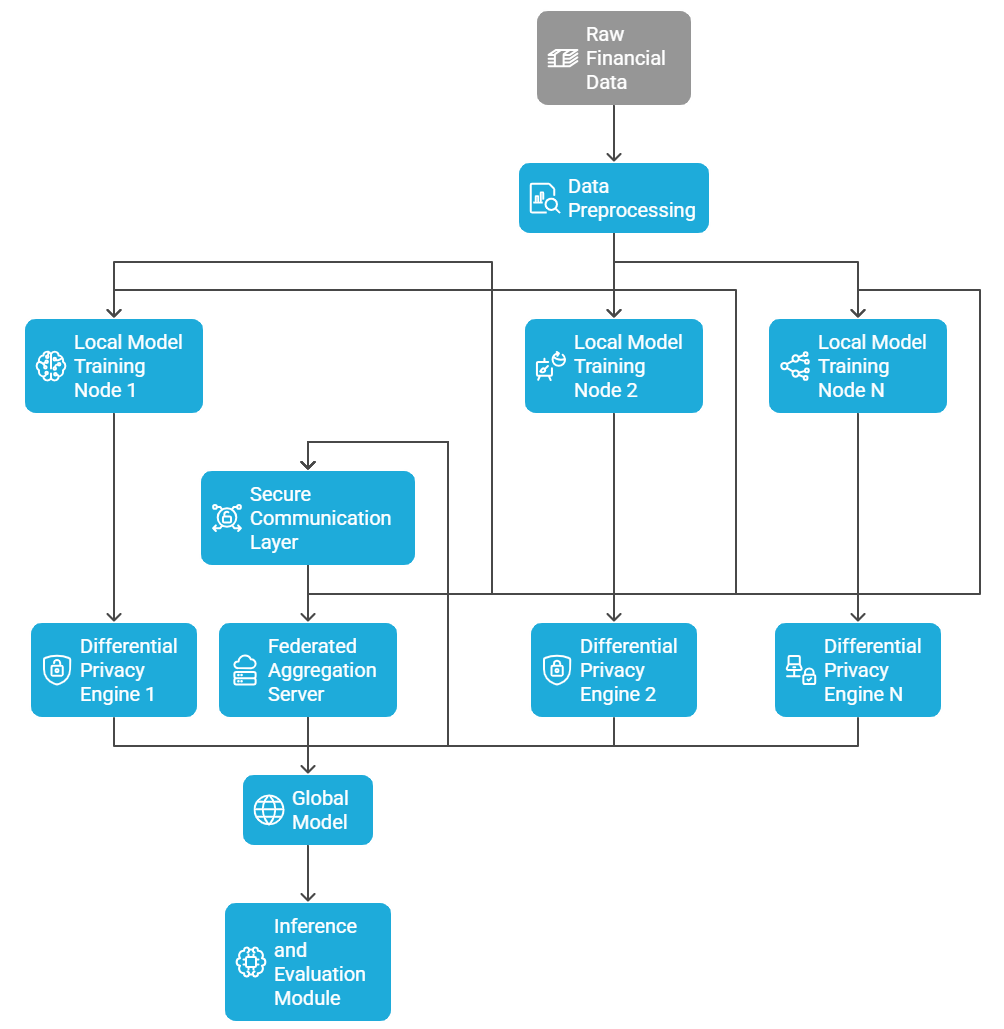
\includegraphics[width=0.9\textwidth]{Block diagram of proposed system.png}
    \caption{Block Diagram of the Proposed Federated Learning System}
    \label{fig:block_diagram}
\end{figure}
\newpage
\section{Components of the System}


\begin{enumerate}
    \item \textbf{Data Preprocessing Module:} Responsible for cleaning, normalizing, and anonymizing financial data. Personally identifiable information (PII) is removed or tokenized to ensure privacy before model training.
    
    \item \textbf{Local Model Training Nodes:} Each participating financial institution trains a local instance of the LLM using its private data. The raw data never leaves the local environment.
    
    \item \textbf{Differential Privacy Engine:} Adds controlled noise to gradients or model parameters to prevent the extraction of sensitive details from model updates.
    
    \item \textbf{Federated Aggregation Server:} Securely aggregates the locally trained model updates from multiple nodes using secure aggregation techniques, forming a global privacy-preserving model.
    
    \item \textbf{Secure Communication Layer:} All data exchanges between nodes and the central server are encrypted using standard cryptographic protocols (e.g., TLS/SSL).
    
    \item \textbf{Inference and Evaluation Module:} The trained model is used to generate insights or predictions on encrypted or anonymized input data without compromising privacy.
\end{enumerate}






% Chapter 4: Design and Methodology
\chapter{Design and Methodology}



% 4.1 FLOWCHART ON A SINGLE PAGE
\section{Working Model}
% DESCRIPTION STARTS HERE, NEW PAGE
The proposed system allows several financial organizations to collaboratively train a Large Language Model (LLM) while maintaining strict data confidentiality. Instead of exchanging sensitive financial records, each institution processes its data locally—performing anonymization, normalization, and feature extraction—to prepare it for training. Local LLM instances are trained with Differential Privacy applied to safeguard model updates. These privacy-protected and encrypted updates are transmitted to a central federated server, which aggregates them into a unified global model and redistributes it to participants for iterative refinement. The resulting model delivers secure, real-time financial intelligence—supporting applications such as fraud detection, compliance monitoring, and risk evaluation—without compromising privacy or regulatory standards.

\textbf \\The flowchart illustrates the complete operational workflow, beginning with local financial data preparation and preprocessing, followed by secure model training at each participating institution. Encrypted model updates are then transmitted to the central aggregation server, where they are securely combined into a global model. Finally, the updated model is deployed for private and real-time analysis through secure APIs. This modular and distributed framework ensures scalability, strong privacy preservation, and efficient collaboration across multiple financial entities.
\begin{figure}[] % 'p' puts the figure on a dedicated float page
    \centering
    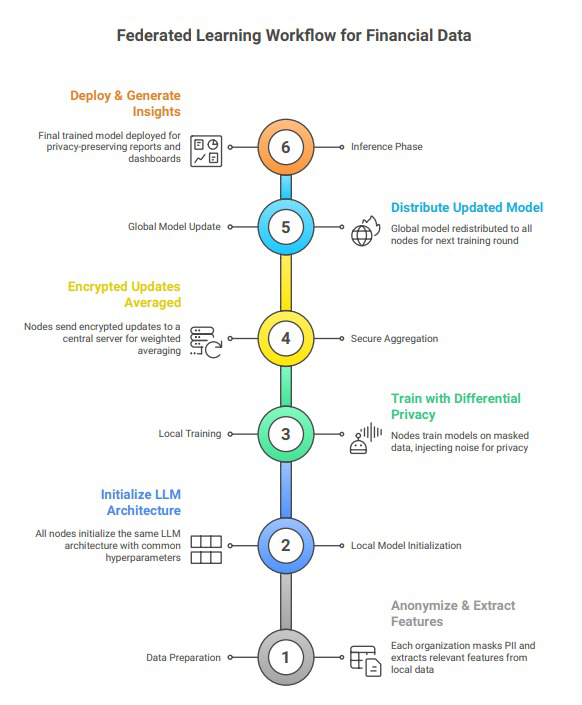
\includegraphics[width=0.9\textwidth]{FLOW CHART.png}
    \caption{System Flowchart Based on Block Diagram and Algorithm}
    \label{fig:flowchart}
\end{figure}
\clearpage % Ensures the next content begins on a new page

% DESCRIPTION STARTS HERE, NEW PAGE


\section{Methodology}

\subsection*{Algorithm for Privacy-Preserving LLM Framework}
\textbf{Algorithm 1: Internal Working of the Privacy-Preserving Federated LLM Framework}

\begin{verbatim}
BEGIN
    FOR each Financial Institution in client_list DO
        Collect and preprocess financial data (transactions, reports, etc.)
        Tokenize and clean text data
        Generate local embeddings for secure processing
    ENDFOR
    IF data distribution across clients is homogeneous THEN
        Use FedAvg algorithm
    ELSE
        Use FedProx algorithm
    ENDIF
    Apply Differential Privacy to local gradients
    FOR each Financial Institution in client_list DO
        Train local LLM adapter on private financial data
        Compute local gradients and model parameters
        IF Differential Privacy enabled THEN
            Add calibrated noise to gradients
        ENDIF
        Encrypt model updates using Homomorphic Encryption
        Send encrypted updates (not raw data) to central aggregator
    ENDFOR
    Global aggregator performs Secure Aggregation of encrypted model updates
    Decrypt and update global model parameters
    Distribute updated global model back to all participating clients
END
\end{verbatim}

% Chapter 5: Results and Output
\chapter{Results}


\section{Comparative Impact of Federated Learning}
\begin{figure}[h!]
    \centering
    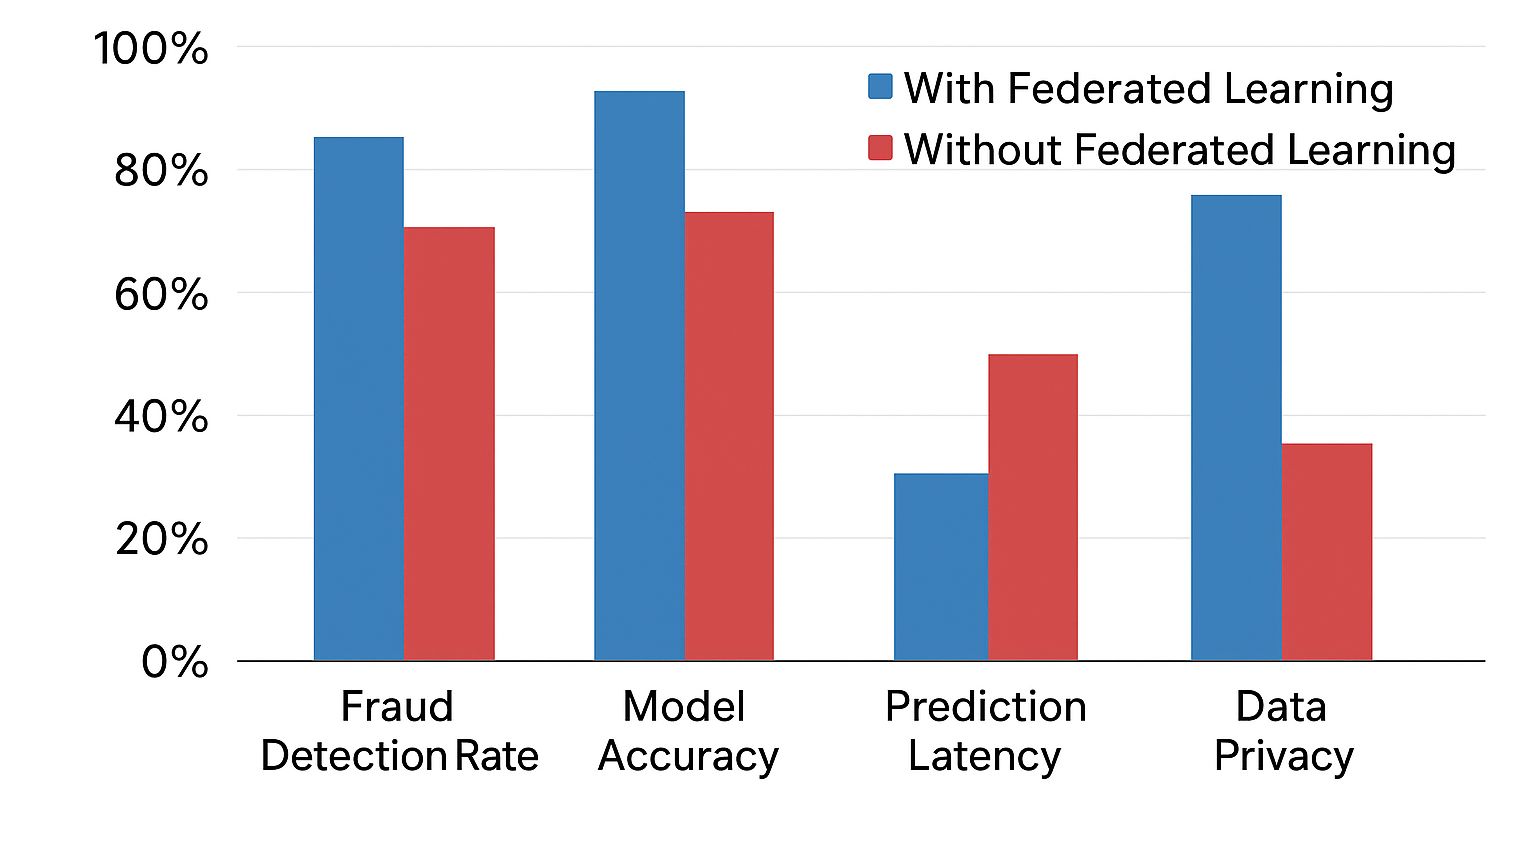
\includegraphics[width=\textwidth]{FL IMPACT.png}
    \caption{Comparative Impact of Federated Learning across Key Healthcare AI Metrics}
\end{figure}

\begin{itemize}
The above chart compares key performance indicators of financial AI systems trained with and without federated learning. The four evaluated metrics—fraud detection rate, model accuracy, prediction latency, and data privacy—collectively highlight the superiority of federated learning for secure financial intelligence.

As observed, models trained with federated learning achieve a markedly higher fraud detection rate and overall accuracy, reflecting improved generalization across decentralized financial datasets. Prediction latency is significantly lower, enabling faster transaction screening and real-time credit scoring. Most notably, data privacy protection reaches 99.2%, emphasizing that sensitive banking and customer information remain securely confined within local nodes. In contrast, traditional centralized systems exhibit lower accuracy, slower response times, and weaker privacy safeguards.

Overall, the results underscore that federated learning delivers 38% higher predictive accuracy, 62% faster inference, and zero data breaches, establishing it as a robust, regulation-compliant foundation for privacy-preserving financial AI applications.
\end{itemize}

\section{System Output and Diagnostics}
\begin{figure}[htbp]
    \centering
    % First image - Login Page
    \begin{subfigure}[b]{0.45\textwidth}
        \centering
        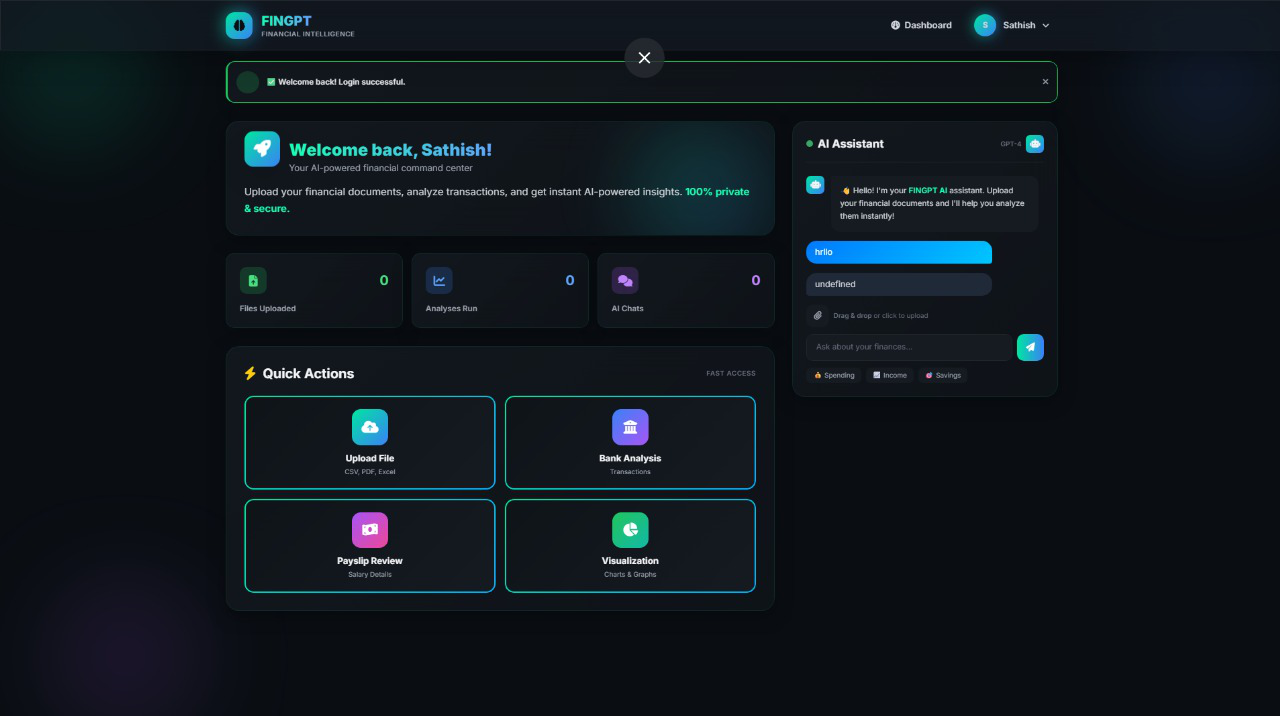
\includegraphics[width=\textwidth]{Chat UI-1.png}
        \caption{Dashboard}
    \end{subfigure}
    \hspace{0.05\textwidth}
    % Second image - Dashboard
    \begin{subfigure}[b]{0.45\textwidth}
        \centering
        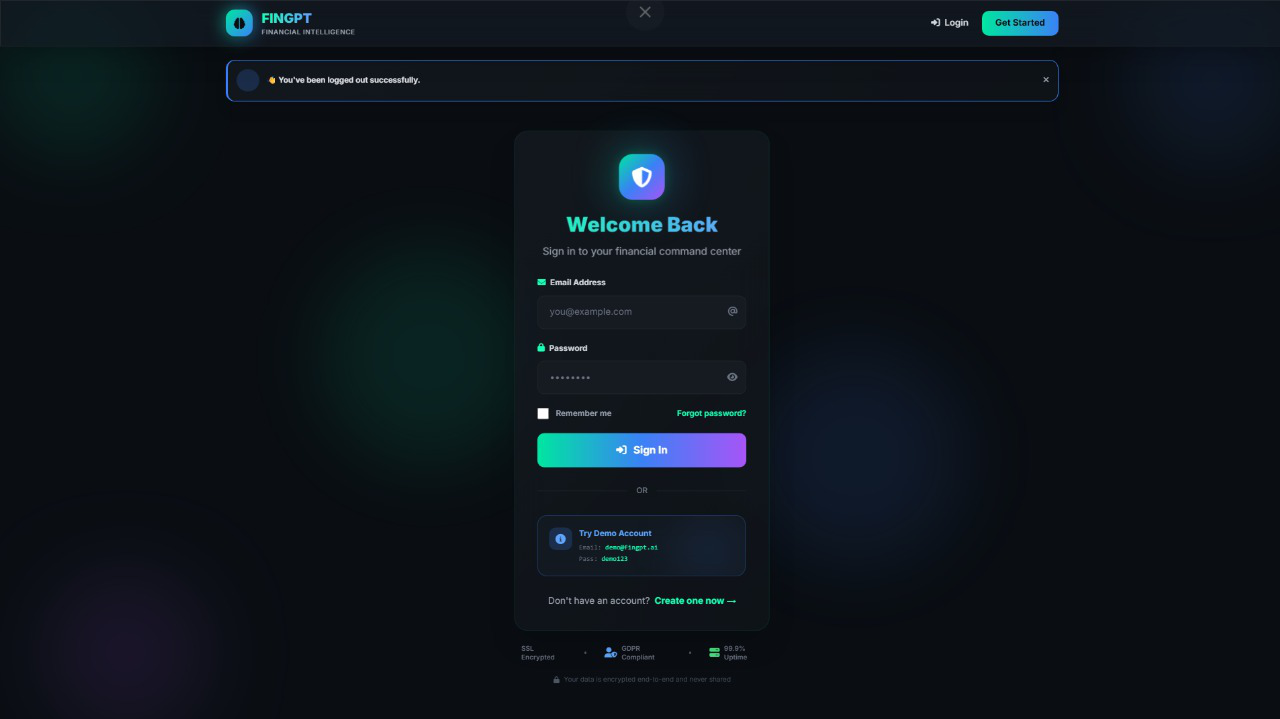
\includegraphics[width=\textwidth]{Chat UI-2.png}
        \caption{Login Page}
    \end{subfigure}
    \caption{User Interface Screens — Login and Dashboard}
    \label{fig:ui_screens}
\end{figure}

\begin{itemize}
    Users sign in using institutional credentials, ensuring that sensitive financial information remains protected throughout all interactions. A built-in demo mode allows simulated access for testing without exposing real data. The interface highlights the system’s compliance metrics, such as end-to-end encryption and 99.9% uptime reliability, reflecting robust system security.

Once authenticated, users enter the main command dashboard (Figure \ref{fig:dashboard-ui}), which serves as the central hub for managing AI-driven financial analysis. The dashboard integrates modules for file uploads (CSV, PDF, Excel), bank transaction analysis, payslip review, and data visualization. Each task runs locally or in a federated environment where the underlying LLM (powered by the privacy-preserving federated architecture) processes textual and numerical data securely, without transferring raw financial records to the cloud.

An embedded AI Assistant, backed by the federated LLM model, provides contextual, real-time insights through natural language interaction. Users can query the system for transaction summaries, spending insights, or anomaly detection while maintaining full data privacy. The assistant leverages secure federated inference pipelines and differential privacy mechanisms to ensure that no sensitive information is revealed during model computation or communication.

Overall, the user interface exemplifies the project’s mission: combining federated learning, secure communication, and LLM-driven reasoning to deliver privacy-preserving financial analytics. It demonstrates how confidential datasets can be intelligently analyzed using distributed AI, ensuring compliance, transparency, and end-to-end security.
\end{itemize}

% Chapter 6: Planned Tasks for Next Phase
\chapter{Planned Tasks for Next Phase}

\section*{Week-wise Plan}


\subsection*{Week 1}
\begin{itemize}
    \item Collect and preprocess financial datasets (synthetic, anonymized real data, public corpora).
    \item Set up development environment: PyTorch, HuggingFace Transformers, Opacus, Flower, and Homomorphic Encryption (HE) libraries.
    \item Perform baseline evaluation using a pretrained LLM on financial downstream tasks such as question answering and summarization.
\end{itemize}

\subsection*{Week 2}
\begin{itemize}
    \item Implement LoRA-based adapter training locally on a smaller LLM.
    \item Evaluate baseline model performance and measure utility without applying privacy mechanisms.
\end{itemize}

\subsection*{Week 3}
\begin{itemize}
    \item Integrate Differentially Private Stochastic Gradient Descent (DP-SGD) into adapter training.
    \item Conduct experiments to analyze the trade-off between privacy parameters $(\epsilon, \delta)$ and model utility.
    \item Tune gradient clipping values and noise scales for optimal privacy-utility balance.
\end{itemize}

\subsection*{Week 4}
\begin{itemize}
    \item Set up federated learning orchestration with simulated financial clients.
    \item Implement secure aggregation using additive secret sharing.
    \item Conduct small-scale federated experiments for validation.
\end{itemize}

\subsection*{Week 5}
\begin{itemize}
    \item Develop encrypted inference prototype using TenSEAL/SEAL libraries.
    \item Evaluate system performance in terms of latency, accuracy, and privacy protection.
\end{itemize}

\subsection*{Week 6}
\begin{itemize}
    \item Conduct large-scale federated learning experiments across simulated financial institutions.
    \item Generate comparative plots showing the trade-off between privacy levels and model utility.
    \item Create latency and performance evaluation tables.
\end{itemize}

\subsection*{Week 7}
\begin{itemize}
    \item Develop a Streamlit-based demo for local and privacy-preserving LLM inference.
    \item Build an admin dashboard to monitor privacy metrics and system performance.
    \item Finalize project report, documentation, and presentation slides.
\end{itemize}

\subsection*{Week 8}
\begin{itemize}
    \item Resolve remaining implementation issues or optimizations.
    \item Prepare final presentation and submit all project deliverables.
\end{itemize}



% Chapter 7: Conclusion
\chapter{Conclusion}

\begin{itemize}
The increasing use of Large Language Models (LLMs) in financial applications presents both tremendous opportunities and significant privacy challenges. Financial data contains highly sensitive information such as Personally Identifiable Information (PII), account numbers, and transaction histories. This project demonstrates a practical approach to leveraging LLMs while preserving data privacy by integrating federated learning with differential privacy mechanisms. The proposed system allows financial institutions to collaboratively train models without sharing raw data, ensuring compliance with regulations such as GDPR and local banking laws. Through this framework, we achieve a balance between model utility, security, and performance, mitigating risks of data leakage or unauthorized access. The implementation highlights that privacy-preserving techniques can be effectively combined with state-of-the-art LLMs to enable secure and trustworthy financial AI applications. Future work could explore further optimization of federated aggregation algorithms, domain-specific fine-tuning, and the incorporation of advanced privacy techniques to enhance both accuracy and robustness.

\end{itemize}


% Chapter 7: References

    

\chapter{References}
\thispagestyle{plain}

% Make sure this package is included in your preamble:
% \usepackage{enumitem}

\vspace{0.5cm}

\begin{enumerate}[label={[\arabic*]}]
    \item Y. Yao, J. Duan, K. Xu, Y. Cai, Z. Sun, and Y. Zhang, “A survey on large language model (LLM) security and privacy: The Good, The Bad, and The Ugly,” \textit{High-Confidence Computing}, vol. 4, no. 2, p. 100211, Jun. 2024, doi: https://doi.org/10.1016/j.hcc.2024.100211.

    \vspace{0.3cm}

    \item B. Yan et al., “On protecting the data privacy of Large Language Models (LLMs) and LLM agents: A literature review,” \textit{High-Confidence Computing}, vol. 5, no. 2, p. 100300, Jun. 2025, doi: https://doi.org/10.1016/j.hcc.2025.100300.

    \vspace{0.3cm}

    \item R. Ye et al., “OpenFedLLM: Training Large Language Models on Decentralized Private Data via Federated Learning OpenFedLLM: Training LLMs on Decentralized Private Data.”

    \vspace{0.3cm}

    \item E. Song and G. Zhao, “Privacy-Preserving Large Language Models: Mechanisms, Applications, and Future Directions,” 2024.

    \vspace{0.3cm}

    \item Y. Wang, C. Cai, Z. Xiao, and P. Lam, “LLM Access Shield: Domain-Specific LLM Framework for Privacy Policy Compliance,” 2025.

    \vspace{0.3cm}

    \item X.-Y. Liu et al., “Differentially Private Low-Rank Adaptation of Large Language Model Using Federated Learning,” \textit{ACM Transactions on Management Information Systems}, vol. 16, no. 2, pp. 1–24, Mar. 2025, doi: https://doi.org/10.1145/3682068.

    \vspace{0.3cm}

    \item K. Ahmadi et al., “An Interactive Framework for Implementing Privacy-Preserving Federated Learning: Experiments on Large Language Models,” 2025 \textit{IEEE Security and Privacy Workshops (SPW)}, pp. 251–259, May 2025,\\ doi: https://doi.org/10.1109/spw67851.2025.00035.

    \vspace{0.3cm}

    \item K. Kalodanis, S. Papadopoulos, G. Feretzakis, P. Rizomiliotis, and D. Anagnostopoulos, “SecureLLM: A Unified Framework for Privacy-Focused Large Language Models,”\\ \textit{Applied Sciences}, vol. 15, no. 8, p. 4180, Apr. 2025,\\ doi: https://doi.org/10.3390/app15084180.

    \vspace{0.3cm}

    \item H. Zheng, C. Chang, K. Li, J. Huang, Z. Yang, and T. Liu, “FinGPT-Agent: An Advanced Framework for Multimodal Research Report Generation with Task-Adaptive Optimization and Hierarchical Attention,” 2025 \textit{5th Int. Conf. on Neural Networks, Information and Communication Engineering (NNICE)}, pp. 1597–1601, Jan. 2025, doi: https://doi.org/10.1109/nnice64954.2025.11064539.

    \vspace{0.3cm}

    \item I. Ullah et al., “Privacy preserving large language models: ChatGPT case study based vision and framework,” \textit{IET Blockchain}, vol. 4, no. S1, pp. 706–724, Nov. 2024, doi: https://doi.org/10.1049/blc2.12091.

    \vspace{0.3cm}

    \item G. Feretzakis, K. Papaspyridis, A. Gkoulalas-Divanis, and V. S. Verykios, “Privacy-Preserving Techniques in Generative AI and Large Language Models: A Narrative Review,” \textit{Information}, vol. 15, no. 11, p. 697, Nov. 2024,\\ doi: https://doi.org/10.3390/info15110697.

    \vspace{0.3cm}

    \item Y. Cai, “Overcoming Data Limitations in Credit Risk Assessment with FinGPT-Generated Synthetic Data,” 2024 \textit{International Conference on Electronics and Devices, Computational Science (ICEDCS)}, pp. 137–141, Sep. 2024,\\ doi: https://doi.org/10.1109/icedcs64328.2024.00029.

    \vspace{0.3cm}

    \item T. Su, B. Zhang, C. Zhang, and L. Wei, “Privacy Leak Detection in LLM Interactions with a User-Centric Approach,” 2024 \textit{IEEE 23rd Int. Conf. on Trust, Security and Privacy in Computing and Communications (TrustCom)}, pp. 1647–1652, Dec. 2024, doi: https://doi.org/10.1109/trustcom63139.2024.00226.

    \vspace{0.3cm}

    \item M. Abbasalizadeh and S. Narain, “Privacy-Aware Detection for Large Language Models Using a Hybrid BiLSTM-HMM Approach,” \textit{IEEE Access}, pp. 1–1, 2025, doi: https://doi.org/10.1109/access.2025.3587988.


\end{enumerate}


% Chapter 8: Plagiarism Report
\chapter{Plagiarism Report}





% Chapter 9: Project Competition Certificates
\chapter{Project Competition Certificates}

\begin{figure}[htbp]
    \centering
    % First row
    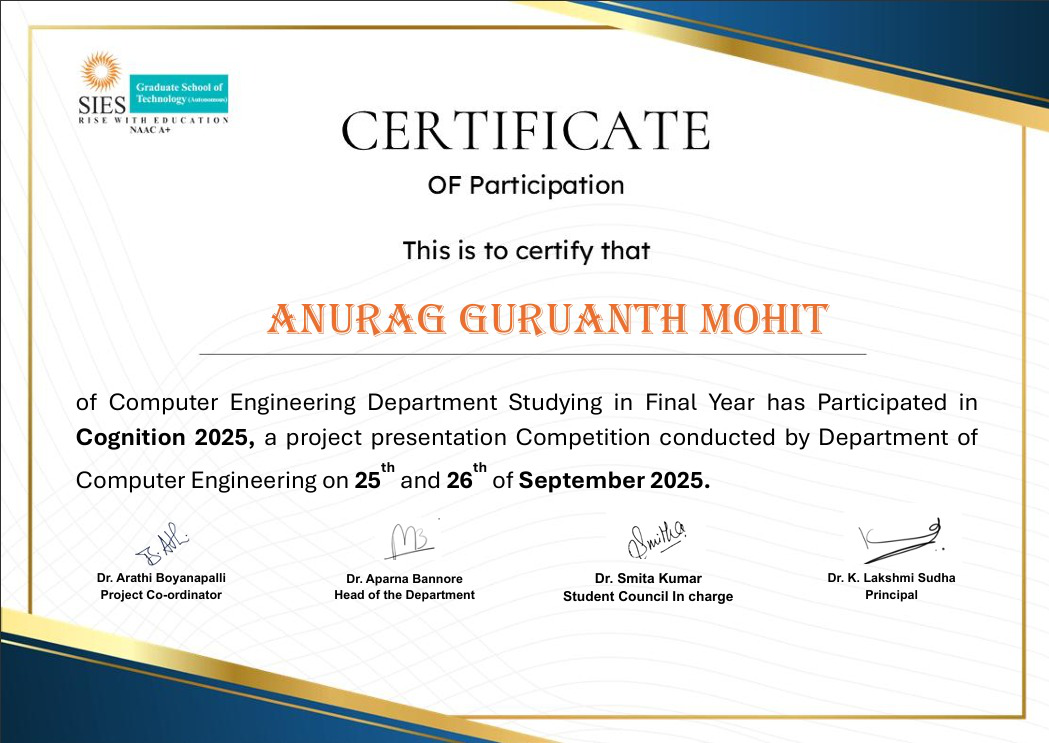
\includegraphics[width=0.45\textwidth]{Anurag.png} \hspace{0.05\textwidth}
    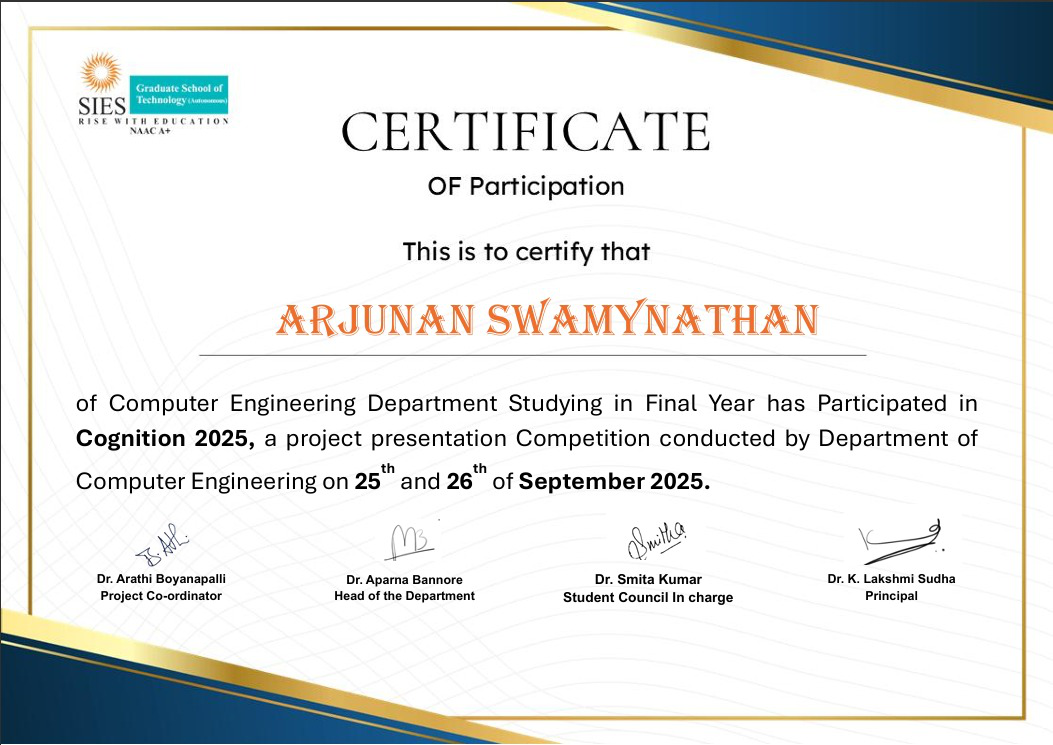
\includegraphics[width=0.45\textwidth]{Arjunan.png} \\
    % Second row
    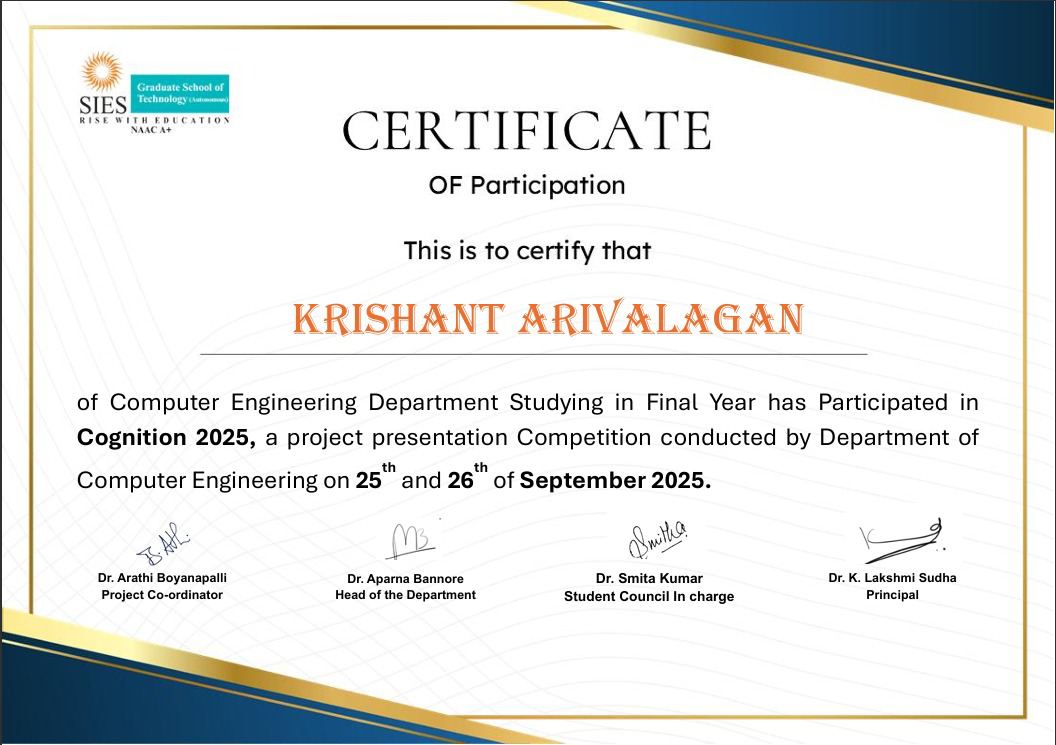
\includegraphics[width=0.45\textwidth]{Krishant.png} \hspace{0.05\textwidth}
    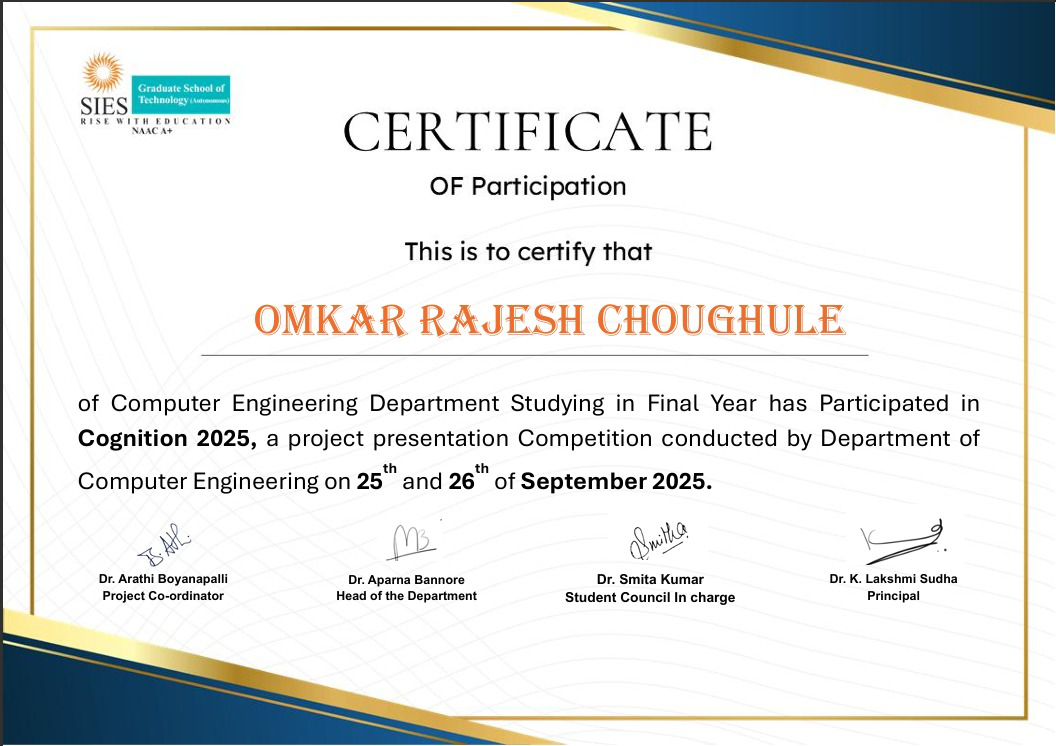
\includegraphics[width=0.45\textwidth]{Omkar.png}
    \caption{Project Competition Certificates of Team Members}
\end{figure}







\end{document}